
\section{Introduction}

This document covers fixed point design. Especially $2$'s complement. 

\section{Fixed Point Concepts}

Fixed point datatypes have a more limited range than floating point numbers. The range is defined by the word-length in bits, position of the binary point (dictates fractional length) and whether the number is signed or unsigned. The position of the binary point dictates scaling and range. \cite{matlab_fxp}.

Note that in the following discussions we will be following the Q format which is defined as Q(IL, FL). Total word length is then $IL + FL + 1$. $IL$ is the integer length and $FL$ is the fractional portion.

Some facts about the fixed point format are as follows
\begin{enumerate}
	\item \textcolor{red}{\textbf{Total Word Length}}: Total word length for signed representation is given by $WL = IL + FL + 1$.
	\item \textcolor{red}{\textbf{Precision}}: The resolution of the representation is given by $\frac{1}{2^{FL}}$.
	\item \textcolor{red}{\textbf{Max value}}: This is given by $2^{IL-1} - \frac{1}{2^{FL}}$. This is intuitively explained as follows. If we have the formal Q(7,8) then the maximum positive value is $01111111.11111111 = 10000000.00000000 - 00000000.00000001$.
	\item \textcolor{red}{\textbf{Min value}}: This is given by $-2^{IL-1}$. This is intuitively 2's complement of $10000000.00000000$.
\end{enumerate}

In MATLAB to create a fixpoint object you can use the `numerictype' keyword.

\begin{lstlisting}[language=matlab]
	>> T2 = numerictype(true, 16, 8)
	>> T2.range

	ans = 

   		1.0e+02 *
  		-1.280000000000000   1.279960937500000

   	DataTypeMode: Fixed-point: binary point scaling
    	Signedness: Signed
        WordLength: 16
        FractionLength: 8
\end{lstlisting}


\subsection{Floating to Fixed point conversion\cite{ucdavis_flt2fxp}}

Everything around us can be described using real number. The problem with real numbers is that you need infinite precision to represent them. We can come close by using IEEE $754$ Floating point format. There are variations to this format such as block floating point etc but we will get to that later. 

To go from floating point numbers to fixed point numbers, you need to do the following steps:
\begin{enumerate}
	\item First multiply by $2^{FL}$.
	\item Then round it. This can be done by adding $0.5$ LSB and then truncating. This will work for both positive and negative numbers.
	\item Truncate by dropping bits after the binary point.
	\item Finally divide by $2^{FL}$. Note that this final step makes sense when you think of this in floating point. In fixed point dividing will lead to bits dropping at the end. By this we mean that divide by $2^{FL}$ only if you want to know what the true decimal value is. In fixed point we dont do this kind of dividing.
\end{enumerate}

Lets take an example. Lets say we have the number $3.456444$ and we want to convert it to fixed point $Q(8, 8)$. Then following these steps you will get the answer $3.45703125$

There is always a need to reduce the number of bits from a larger to smaller number. This is very typical in DSP applications where say you are adding or multiplying numbers. There is always a bit-growth and you eventually want to bring them down to the same number of bits as the input. Before we get into the topics of Saturation and Rounding, we will take a brief detour to the topic of bit-growth.
 
\subsection{Bit-Growth \cite{zipcpu_bitgrowth}}

When we add, subtract and multiply numbers in fixed point, we always have bit-growth in the result. So the question becomes, ``By how much should I increase word-length of the output so as to avoid overflow?''. There are some general rules to remember when you do add/subtract and multiply (Remember division is just a multiply too). 

The range of a 2's complement number is
\[
-2^{N-1} \leq a \leq 2^{N-1}-1 
\]

For unsigned numbers this range is
\[
0 \leq a \leq 2^{N}-1 
\]

\subsubsection{Addition/Subtraction}

If we do $K$ additions of $N$-bit numbers, the final result will need $N + log_2(K)$ bits. Its actually fun to derive this result \cite{zipcpu_bitgrowth}. We can derive it by adding $K$ extreme values.

\begin{equation} \label{eq1}
		Sum = K \times 2^{N-1}-1
\end{equation}

Lets assume a number $M$ that represents the number of bits to represent $K$. We want this $M$ to be as tight as possible. This means we want
\[
	K \leq 2^M
\]

Taking log on both sides we get
\[
	log_2(K) \leq M 
\]

So the tightest $M$ we can get is: 

\[
	M = \lceil log_2(K) \rceil
\]

Therefore, the total number of bits needed for the final answer is 
\begin{equation}
	Number\; of \; bits = \textcolor{red}{N + log_2(K)}
\end{equation}

\subsubsection{Multiplication}

When you multiply two numbers of length $N$ and $M$, the output will need $N+M-1$ bits. Deriving this is easy. Multiply out the extremes. 

\[
[2^{N-1}-1] \times [2^{M-1}-1] = 2^{N+M-2} - 2^{M-1} - 2^{N-1} + 1 \leq 2^{N+M-1} 
\]

You can show the same on the negative extremes. 

The number of bits needed at the output is 
\begin{equation}
	Number \; of \; bits = \textcolor{red}{N+M-1}
\end{equation}


\subsection{Saturation \cite{ucdavis_sat}}

There are mainly two techniques to reduce the bit-size. One is saturation and other is rounding (next section). Saturation is when we want to remove MSB bits. We wa


This discussion is based on the description given in \cite{ucdavis_sat}. Basically saturation is a 3-input mux that does the following checks

\begin{enumerate}
	\item in $>$ SAT\_HI or in $\geq$ SAT\_HI
	\item in $<$
\end{enumerate}






\section{Email Discussions}

\subsection{Signed multiplication}

Hi,
I am looking through some of the mult implementation in the RTL code that is part of the lane processing in the LCU.
Right now the way its implemented is the mult module takes 2x32 bit operands. It then breaks it down into 4 bytes each. Before it does the break up however, it converts the operands to absolute values. This is done based on the datatype. For instance if the datatype is S8, then a given operand will have 4 of these samples. Each sample is converted to its absolute value via 2's complement. Now you have positive values for each byte and these are all multiplied out to form partial products. 
Now from here depending on what kind of multiplication we are doing, we use the partial products to form the final result. This is done via shifting and adding of the partial products. Once the final result is formed, we check to see the sign of the operands and if either one is negative, we do a negate. 
I looked at the negation code and it looked like this:
 
	\begin{figure}[h]
		\centering
  		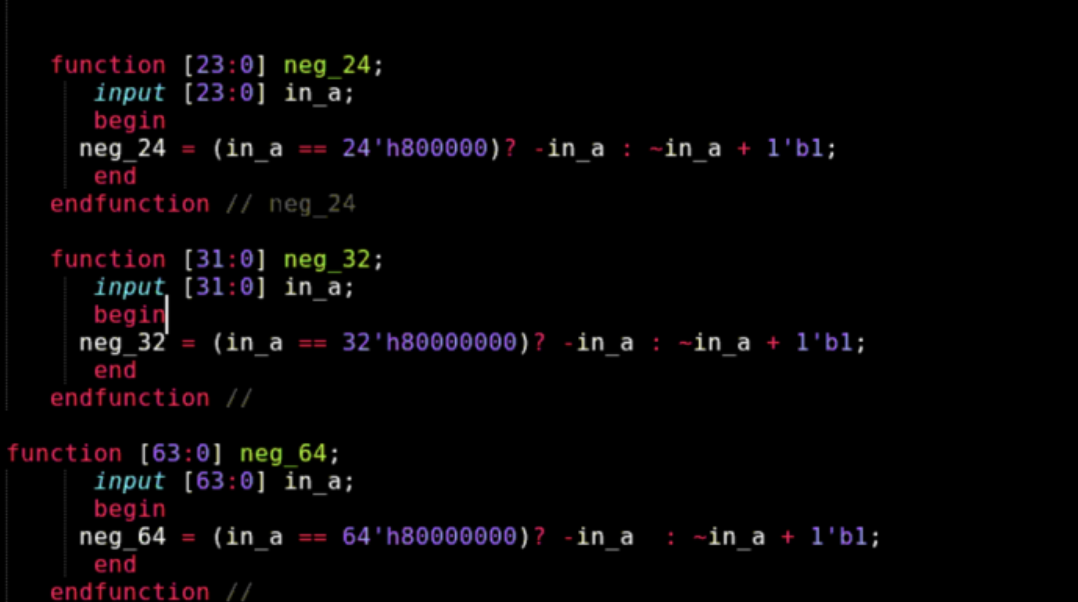
\includegraphics[width=0.8\linewidth]{SignedMul.png}
  		\caption{Signed Multiplication Code}
  		\label{fig:SignedMul}
  	\end{figure} 

Lets take an example of S8 by S8 multiplication. The following are the steps1) Convert each S8 sample to its positive value2) Multiply the two positive values to form a 16 bit number3) check if any one of the S8 sample was negative and then negate the result in step 2 if either of the operands is. This would be done using the $neg16$ function above.
If you see this function its does a check for 16'h8000 which in decimal is 32768. I am not sure why this is done. If you look at s8 numbers, the range is -128 to 127. You are then taking absolute values and multiplying. When multiplying two s8 numbers, the max negative value is -127*128 = -16256 and the max positive value you can get is -128 x -128 = 16384. So according to the algorithm above for the most negative result you will get $16256$ which you would negate. My contention is that you will never get to that check that is being done. This is an unnecessary MUX in the path. Though it looks very trivial to leave it there, the problem is i am trying to increase the clock rate and I would like to remove any redundant logic thats not really needed. 




























\newpage
 \printbibliography
